%%%%%%%%%%%%%%%%%%%%%%%%%%%%%%%%%%%%%%%%%%%%%%%%%%%%%%%%
% Este é um documento que servirá de modelo para
% os relatórios feitos na disciplina Laboratório de Circuitos Lógicos
% 2020-2
%%%%%%%%%%%%%%%%%%%%%%%%%%%%%%%%%%%%%%%%%%%%%%%%%%%%%%%%%

%%%%%%%%%%%%%%%%%%%%%%%%%%%%%%%%%%%%%%%%%%%%%%%%%%%%%%%%%
% Use os diferentes diretórios para colocar os relatórios de cada experimento, deste modo vc consegue manter um histórico e todo material organizado em apenas um local.
% Lembre-se de mudar o Main Document no Menu!!!

\documentclass[12pt]{article}

\usepackage{sbc-template}
\usepackage[brazil,american]{babel}
\usepackage[utf8]{inputenc}

\usepackage{graphicx}
\usepackage{url}
\usepackage{float}
\usepackage{listings}
\usepackage{color}
\usepackage{todonotes}
\usepackage{algorithmic}
\usepackage{algorithm}
\usepackage{hyperref}
\usepackage{amsmath}
\usepackage{graphicx}
\usepackage{array}
\usepackage{mwe}
\usepackage[shortlabels]{enumitem}

\usepackage{xcolor}
\usepackage{listings}
\definecolor{vgreen}{RGB}{104,180,104}
\definecolor{vblue}{RGB}{49,49,255}
\definecolor{vorange}{RGB}{255,143,102}

\lstdefinestyle{verilog-style}
{
    language=Verilog,
    basicstyle=\small\ttfamily,
    keywordstyle=\color{vblue},
    identifierstyle=\color{black},
    commentstyle=\color{vgreen},
    numbers=left,
    numberstyle=\tiny\color{black},
    numbersep=10pt,
    tabsize=8,
    moredelim=*[s][\colorIndex]{[}{]},
    literate=*{:}{:}1
}

\makeatletter
\newcommand*\@lbracket{[}
\newcommand*\@rbracket{]}
\newcommand*\@colon{:}
\newcommand*\colorIndex{%
    \edef\@temp{\the\lst@token}%
    \ifx\@temp\@lbracket \color{black}%
    \else\ifx\@temp\@rbracket \color{black}%
    \else\ifx\@temp\@colon \color{black}%
    \else \color{vorange}%
    \fi\fi\fi
}
\makeatother

\usepackage{trace}

\sloppy


\title{Experimento 7\\
Latches e Flip-Flops: RS e JK}

\author{Matheus Cardoso de Souza, 202033507\\
        Ualiton Ventura da Silva, 202033580\\
        Grupo G42
}

%%%% LEMBRE-SE DE MUDAR O GRUPO NA LINHA ABAIXO!!!!! %%%%%%
\address{Dep. Ciência da Computação -- Universidade de Brasília (UnB)\\
  CIC0231 - Laboratório de Circuitos Lógicos
  \email{matheus-cardoso.mc@aluno.unb.br, 202033580@aluno.unb.br}
}

\begin{document}
\maketitle

\selectlanguage{american}
 \begin{abstract}
   The current report explores the construction of different models of
   \emph{Latches} and \emph{Flip-flops}, showing their specificities, utilities
   and inherent limitations. Such circuits, so widely used to build up
   computational circuits, show themselves as vital for the modern society, and,
   therefore, it's thorough study and understanding becomes of crucial
   importance for Computer Science students.
 \end{abstract}

\selectlanguage{brazil}
 \begin{resumo}
   O presente relatório aborda a construção de \emph{Latches} e
   \emph{Flip-flops} de diferentes modelos, explorando suas especificidades,
   utilidades e limitações inerentes. Tais circuitos, tão amplamente utilizados
   para a construção de circuitos computacionais atuais, mostram-se de vital
   importancia para a sociedade moderna, e, portanto, seu estudo minucioso
   apresenta-se como um imperativo para estudantes de Ciências da Computação.
 \end{resumo}


\section{Introdução}\label{sec:Introducao}

A princípio existem variados tipos de métodos utilizados para o registro de
memória, mas os experimentos realizados visam descrever e utilizar aqueles que
surgem do uso de semicondutores.

Com o uso de portas lógicas podem haver outras maneiras além da que será descrita
no presente relatório, assim como um mesmo sistema de memória poderá ser
descrito com diferentes portas lógicas. Por exemplo, um Latch RS poderá ser
representado tanto com o uso de portas \emph{NAND} como \emph{NOR}, contudo, nos
experimentos realizados optou-se pelo uso de portas \emph{NAND}.

\subsection{Objetivos}\label{sec:Objetivos}
Apesar da existência de outros sistemas de memória, focou-se na elaboração e
análise de Latch RS Simples, Latch RS Engatilhado, Flip Flop RS e Flip Flop JK.

É necessário notar que diante das análises de cada circuito de memória, alguns
possuem estados proibidos e estes mesmos estados serão explorados mais a
adiante.

\subsection{Materiais}\label{sec:Materiais}

Em função da natureza do ensino a distância, os presentes experimentos não foram
realizados usando-se materiais e equipamentos físicos, mas sim emulados por meio
do software
\href{https://www.digitalelectronicsdeeds.com/downloads.html}{Deeds}.

A seguir estão enumerados os materiais utilizados:
\begin{itemize}
    \item Software Deeds
    \item Portas lógicas
    \begin{itemize}
      \item \emph{OR}
      \item \emph{NOT}
      \item \emph{NAND}s de $2$ e $3$ entradas
    \end{itemize}
    \item \emph{Clocks}
    \item \emph{LED}s
\end{itemize}

\section{Procedimentos}\label{sec:Procedimentos}
% \setcounter{subsection}{-1}

Passaremos a apresentar os experimentos requeridos.

% 2.1
\subsection{Latch RS simples com \textbf{NAND}s}\label{sec:2.1}

Para esta primeira parte do experimento, desejamos implementar um circuito que
seja semelhante ao diagrama da figura~\ref{fig:diagram_2.1.png}.

\begin{figure}[H]
  \centering
  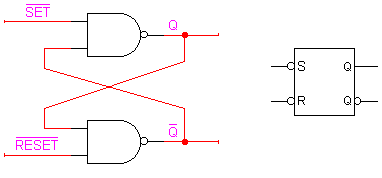
\includegraphics[width=0.5\textwidth]{Exp07/Images/diagram_2.1.png}
  \caption{Latch RS (implementado com \emph{NAND}s)}\label{fig:diagram_2.1.png}
\end{figure}

Com base em~\cite{cl_latchs_RS_D} sabemos que a tabela verdade para o circuito
de uma \emph{Latch RS} deve ser igual à expressa na
tabela~\ref{tab:truth_table_latch_rs}. Assim, temos como proposta de
implementação o circuito demonstrado em~\ref{fig:Circ-2.1.png}.

\begin{table}[H]
    \centering
    \caption{Tabela Verdade para \emph{Latch RS}}
    \begin{tabular}{|c|c||c|c|}\hline
      \multicolumn{2}{|c||}{Entradas} & \multicolumn{2}{|c|}{Saídas} \\\hline
      \textbf{A $(\overline{RESET})$} & \textbf{B $(\overline{SET})$} & \textbf{L0 $(Q)$} & \textbf{L1 $(\overline{Q})$} \\\hline
      0 & 0 & 1 & 1 \\\hline
      0 & 1 & 1 & 0 \\\hline
      1 & 0 & 0 & 1 \\\hline
      1 & 1 & $Q_{n}$ & $\overline{Q_{n}}$ \\\hline
    \end{tabular}\label{tab:truth_table_latch_rs}
\end{table}

\begin{figure}[H]
  \centering
  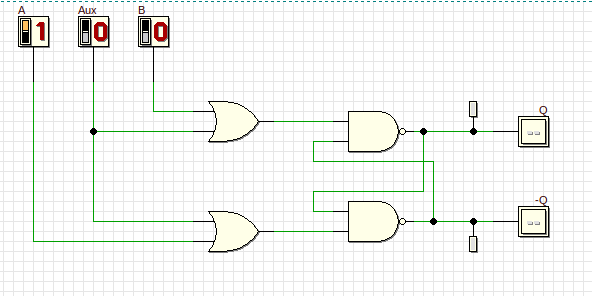
\includegraphics[width=0.5\textwidth]{Exp07/Images/Circ-2.1.png}
  \caption{Latch RS (implementado com \emph{NAND}s)}\label{fig:Circ-2.1.png}
\end{figure}

É interessante notar que o circuito em~\ref{fig:Circ-2.1.png} não é exatamente
igual ao do diagrama em~\ref{fig:diagram_2.1.png} pois a passagem dos estados
$11 \rightarrow 00 \rightarrow 11$ seria difícil de reproduzir manualmente.
Dessa forma, foi adicionado um input adicional e duas portas \emph{OR} para
permitir uma transição mais exata entre esses estados.

Para a visualização do funcionamento deste circuito, confira no seguinte link:
\href{https://youtu.be/RH6w3QnfUhA}{https://youtu.be/RH6w3QnfUhA}

% 2.2
\subsection{Latch RS engatilhado}\label{sec:2.2}

Utilizando os modelos de circuitos apresentados temos que sua implementação
através do software Deeds será:

\begin{figure}[H]
  \centering
  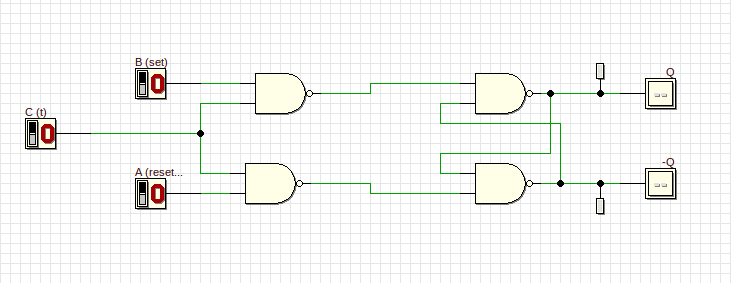
\includegraphics[width=0.8\textwidth]{Exp07/Images/Circ-2.2.png}
  \caption{Latch RS Engatilhado (implementado com \emph{NAND}s)}\label{fig:LatchRS-Engatilhado.png}
\end{figure}

Sendo que a tabela verdade utilizada será:
\begin{table}[H]
    \centering
    \caption{Tabela Verdade para \emph{Latch RS Engatilhado}}
    \begin{tabular}{|c|c|c||c|c|}\hline
      \multicolumn{3}{|c||}{Entradas} & \multicolumn{2}{|c|}{Saídas} \\\hline
      \textbf{C $({TRIGGER})$} & \textbf{A $({RESET})$} & \textbf{B $({SET})$} & \textbf{L0 $(Q_{n+1})$} & \textbf{L1 $(\overline{Q_{n+1}})$} \\\hline
      0 & X & X & $Q_{n}$ & $\overline{Q_{n}}$ \\\hline
      1 & 0 & 0 & $Q_{n}$ & $\overline{Q_{n}}$\\\hline
      1 & 0 & 1 & 0 & 1\\\hline
      1 & 1 & 0 & 1 & 0 \\\hline
      1 & 1 & 1 & 1 & 1 \\\hline
    \end{tabular}\label{tab:truth_table_latch_rs_triggered}
\end{table}

A utilização de um gatilho permite definir quando poderá ocorrer o registro de
bits ou não, portanto para $T=0$, temos que o estado das saídas não poderá ser
modificado, caso contrário temos a situação em que $T=1$, sendo que este caso
descrito possuirá o mesmo comportamento ao utilizar um Latch RS comum.

Para a visualização do funcionamento deste circuito, confira no seguinte link:
\href{https://youtu.be/VNXkBLNcpbo}{https://youtu.be/VNXkBLNcpbo}

% 2.3
\subsection{Flip-flop RS}\label{sec:2.3}

Implementando o circuito através do software Deeds, temos:
\begin{figure}[H]
  \centering
  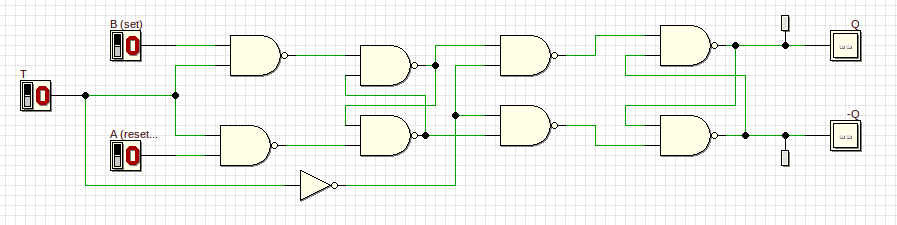
\includegraphics[width=0.8\textwidth]{Exp07/Images/Circ-2.3.png}
  \caption{Flip Flop RS (implementado com \emph{NAND}s)}\label{fig:Flip-Flop-RS.png}
\end{figure}

Simulando tem-se o seguinte comportamento:
\href{https://youtu.be/qPIkTOfm8uI}{https://youtu.be/qPIkTOfm8uI}

Assim, sua tabela verdade será descrita por:
\begin{table}[H]
    \centering
    \caption{Tabela Verdade para \emph{Flip-flop RS}}
    \begin{tabular}{|c|c|c||c|c|}\hline
      \multicolumn{3}{|c||}{Entradas} & \multicolumn{2}{|c|}{Saídas} \\\hline
      \textbf{C $({TRIGGER})$} & \textbf{A $({RESET})$} & \textbf{B $({SET})$} & \textbf{L0 $(Q_{n+1})$} & \textbf{L1 $(\overline{Q_{n+1}})$} \\\hline
      0 & X & X & $Q_{n}$ & $\overline{Q_{n}}$ \\\hline
      $Clk_H$ & 0 & 0 & $Q_{n}$ & $\overline{Q_{n}}$\\\hline
      $Clk_H$ & 0 & 1 & 0 & 1\\\hline
      $Clk_H$ & 1 & 0 & 1 & 0 \\\hline
      $Clk_H$ & 1 & 1 & 1 & 1 \\\hline
    \end{tabular}\label{tab:truth_table_flipflop_rs}
\end{table}

Em questão de saídas poderá não parecer perceptível a diferença entre Latches e
Flip Flops, contudo, um fator imprescindível entre ambos é o fato de que Latches
para que possam criar sua mudança de estado, basta que o nível mude para um que
possibilite esta mudança. Já Flip Flops, possuem a característica de que
para criar suas mudanças será possível somente nas bordas da onda, ou seja, um
flip flop sensível a onda de subida somente modificará seu estado no momento em
que ocorre a transição de nível lógico baixo para alto, assim, define-se que
Latches são sensível ao estado lógico, diferentemente de flip flops que são
sensíveis às bordas.

% 2.4
\subsection{Flip-flop JK}\label{sec:2.4}

Temos que seu circuito será descrito no software Deeds como:

\begin{figure}[H]
  \centering
  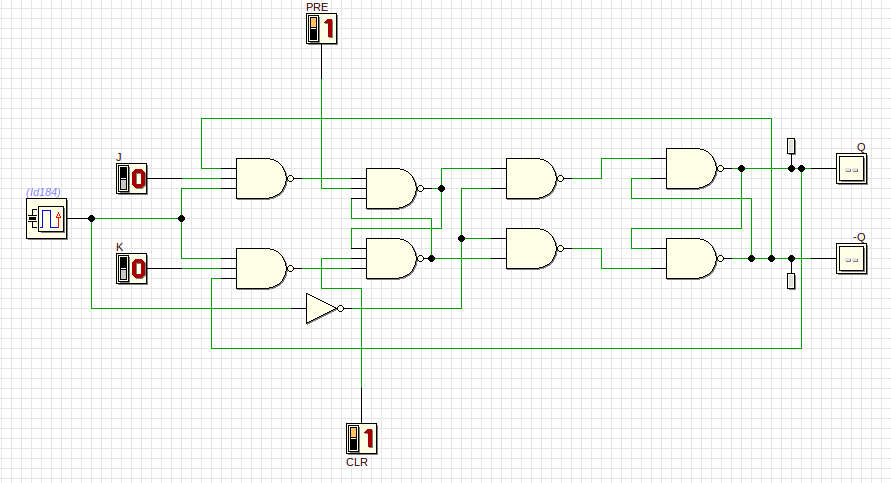
\includegraphics[width=0.7\textwidth]{Exp07/Images/Circ-2.4.png}
  \caption{Flip Flop JK (implementado com \emph{NAND}s)}\label{fig:flip-flop-jk.png}
\end{figure}

Observe que para sua implementação fez-se necessário o uso de entradas de
\emph{PRESET} e \emph{CLEAR}, por não haver estado inicial definido. Contudo,
não utilizou-se a entrada de \emph{CLEAR}, mas definiu-se para ser possível a
criação de um modelo mais completo. Simulando obtemos o seguinte funcionamento: 

\href{https://youtu.be/QCF_M5kqSQE}{https://youtu.be/QCF_M5kqSQE}

Este mesmo \emph{Flip Flop} poderá ser utilizado como um divisor de frequência
de maneira que possa diminuir a frequência de um determinado clock. Segue abaixo
o vídeo que descreve seu comportamento:

\href{https://youtu.be/00iOIssj00k}{https://youtu.be/00iOIssj00k}

Analisando de maneira geral, medindo 1 pulso de $Q$, obtemos:
\begin{figure}[H]
  \centering
  \includegraphics[width=0.7\textwidth]{Exp07/Images/Simul5_2.4.png}
  \caption{Medida de Saída em Q}\label{fig:flip-flop-jk-q.png}
\end{figure}

Analisando 1 pulso de $T$, obtemos:
\begin{figure}[H]
  \centering
  \includegraphics[width=0.8\textwidth]{Exp07/Images/Simul6_2.4.png}
  \caption{Medida de Saída em T}\label{fig:flip-flop-jk-t.png}
\end{figure}

Como 1 pulso nos exemplos utilizados descrevem a metade de um período, temos
então que seus períodos serão aproximadamente:

    $P_{Q} \approx 200ns$
    
    $P_{T} \approx 100ns$
    
Logo:

    $F_{Q} \approx \frac{1}{P_{Q}} \approx 0.005(ns^{-1})$
    
    $F_{T} \approx \frac{1}{P_{T}} \approx 0.01(ns^{-1})$
    
Calculando suas razões:
    
    $\frac{F_{Q}}{F_{T}} = 0,5$
    
Assim, concluimos que a frequência de Q é metade da de T.


\section{Análise dos Resultados}\label{sec:resultados}

Passaremos a analisar individualmente cada um dos tópicos anteriores, levantando
observações pertinentes para cada um deles.

\subsection{Análise do tópico~\ref{sec:2.1}}\label{sec:analise2.1}

No tópico~\ref{sec:2.1} podemos fazer uma observação que se repetirá nos
tópicos~\ref{sec:2.2} e~\ref{sec:2.3}, que é referente a questão de
\emph{estados proibidos}. Como é possível perceber no
\href{https://youtu.be/RH6w3QnfUhA}{vídeo} deste experimento, quando há a
transição do estado $00$ para o estado $11$, o software \emph{Deeds}, que simula
os circuitos digitais, levanta um erro de ``loop infinito''. Esse comportamento
ocorre pois, no estado $00$ o circuito entra no \emph{estado proibido} pois, em
um circuito real, após sair desse estado, a transição se dará de forma não
determinística, sendo dependente de atrasos causados por fios e portas lógicas
que compões o \emph{Latch RS} em específico. No caso do simulador \emph{Deeds},
como não há atrasos de portas lógicas sendo simulado, o programa acaba por
emular ambos $Q$ e $\overline{Q}$ indo para o estado oposto quando $SET$ e
$RESET$ são postos em $1$. Dessa forma, haverá uma eterna mudança entre os
estados $\{Q = 1, \overline{Q} = 1\}$ e $\{Q = 0, \overline{Q} = 0\}$. Dessa
forma, o programa para a execução levantando o erro de ``loop infinito''.

Tal problema não aconteceria com outros circuitos, como por exemplo
\emph{Latches D}, assim como explicado em~\cite{cl_latchs_RS_D}, nem em
\emph{Flip-flops D/JK} como mencionado em~\cite{cl_flipflops_RS_D_JK} e nem em
\emph{Flip-flops T} assim como ensinado em~\cite{cl_flipflop_T_clear_preset}.

\subsection{Análise do tópico~\ref{sec:2.2}}\label{sec:analise2.2}

Semelhantemente ao experimento feito em~\ref{sec:2.1}, temos que o \emph{estado
  proibido} está presente caso \emph{SET} e \emph{RESET} assumam o valor $1$ ao
mesmo tempo. E, dessa forma, ao mudar ambos para o valor $0$ ao mesmo tempo, o
circuito entra em estado não determinístico. E, uma vez que o \emph{Deeds} não
simula atraso aleatório inerente à portas lógicas e cabos usados para construção
do circuito, o programa entra num estado de ``loop infinito'', alternando entre
estados de $0$ e $1$. Dessa forma, ele interrompe a execução da emulação
levantando um erro.

\subsection{Análise do tópico~\ref{sec:2.3}}\label{sec:analise2.3}

A utilização de um Flip Flop e Latch RS possibilitou observar as diferenças
contrastantes entre Flip Flops e Latches. E pode-se comprovar seus
comportamentos.

\subsection{Análise do tópico~\ref{sec:2.4}}\label{sec:analise2.4}

Com o Flip Flop JK descrito, foi possível não somente a análise de seu
funcionamento como o esperado assim como também a sua utilização para a criação
de um divisor de frequência, podendo ser feita uma análise que buscava comprovar
e evidenciar o comportamento divisor.

Deve-se atentar ao fato de que para aumentar as divisões bastaria criar um
comportamento em série de vários Flip Flops JK.

\section{Conclusão}\label{sec:Conclusao}

Através dos experimentos realizados pudemos descrever parcialmente o
comportamento de circuitos utilizados para o armazenamento de memória, assim
como também pudemos analisar o erro associado aos mesmos.

Pode-se observar que circuitos sequencias podem ser utilizados não somente para
o armazenamento de dados, mas também como controle de pulsos de clock e ainda
serem empregados em circuitos como de divisores de frequências.

\nocite{*}
\bibliographystyle{sbc}
\bibliography{relatorio}  %Aqui é a definição do arquivo .bib a ser usado pelas referências


\newpage
% Colocar aqui apenas as respostas dos itens da Auto-Avaliação
\section*{Auto-Avaliação}

Respostas:

\begin{table}[H]
      \begin{tabular}{|c|c|} \hline
      \textbf{Questão} & \textbf{Resposta}\\
      \hline
      1  & D \\ \hline
      2  & A \\ \hline
      3  & B \\ \hline
      4  & D \\ \hline
      5  & C \\ \hline
      6  & D \\ \hline
      7  & D \\ \hline
      \end{tabular}
\end{table}


\end{document}
